% ============================================================================
%  JevGAG + DDAG architecture figure
%  PRIOR STUDY -> PART 1 (report) -> PART 2 (method); one row per precondition,
%  showing the boundary found and how this work resolves it.  Jev thread highlighted.
%  Compile: pdflatex (MiKTeX).
% ============================================================================
\documentclass[border=6pt]{standalone}
\usepackage[T1]{fontenc}
\usepackage{helvet}
\renewcommand{\familydefault}{\sfdefault}
\usepackage{tikz}
\usetikzlibrary{arrows.meta,positioning,fit,backgrounds,calc}
\usepackage{xcolor}

\definecolor{ink}{HTML}{1A2233}
\definecolor{muted}{HTML}{5A6B80}
\definecolor{line}{HTML}{C9D4E2}
\definecolor{priorc}{HTML}{6B7A90}
\definecolor{reportc}{HTML}{1668D6}
\definecolor{methodc}{HTML}{0F9D76}
\definecolor{jevc}{HTML}{B26A00}
\definecolor{bandbg}{HTML}{FFF6E6}
\definecolor{rowbg}{HTML}{F6F9FC}

\begin{document}
\hyphenpenalty=10000
\exhyphenpenalty=10000
\tolerance=2000
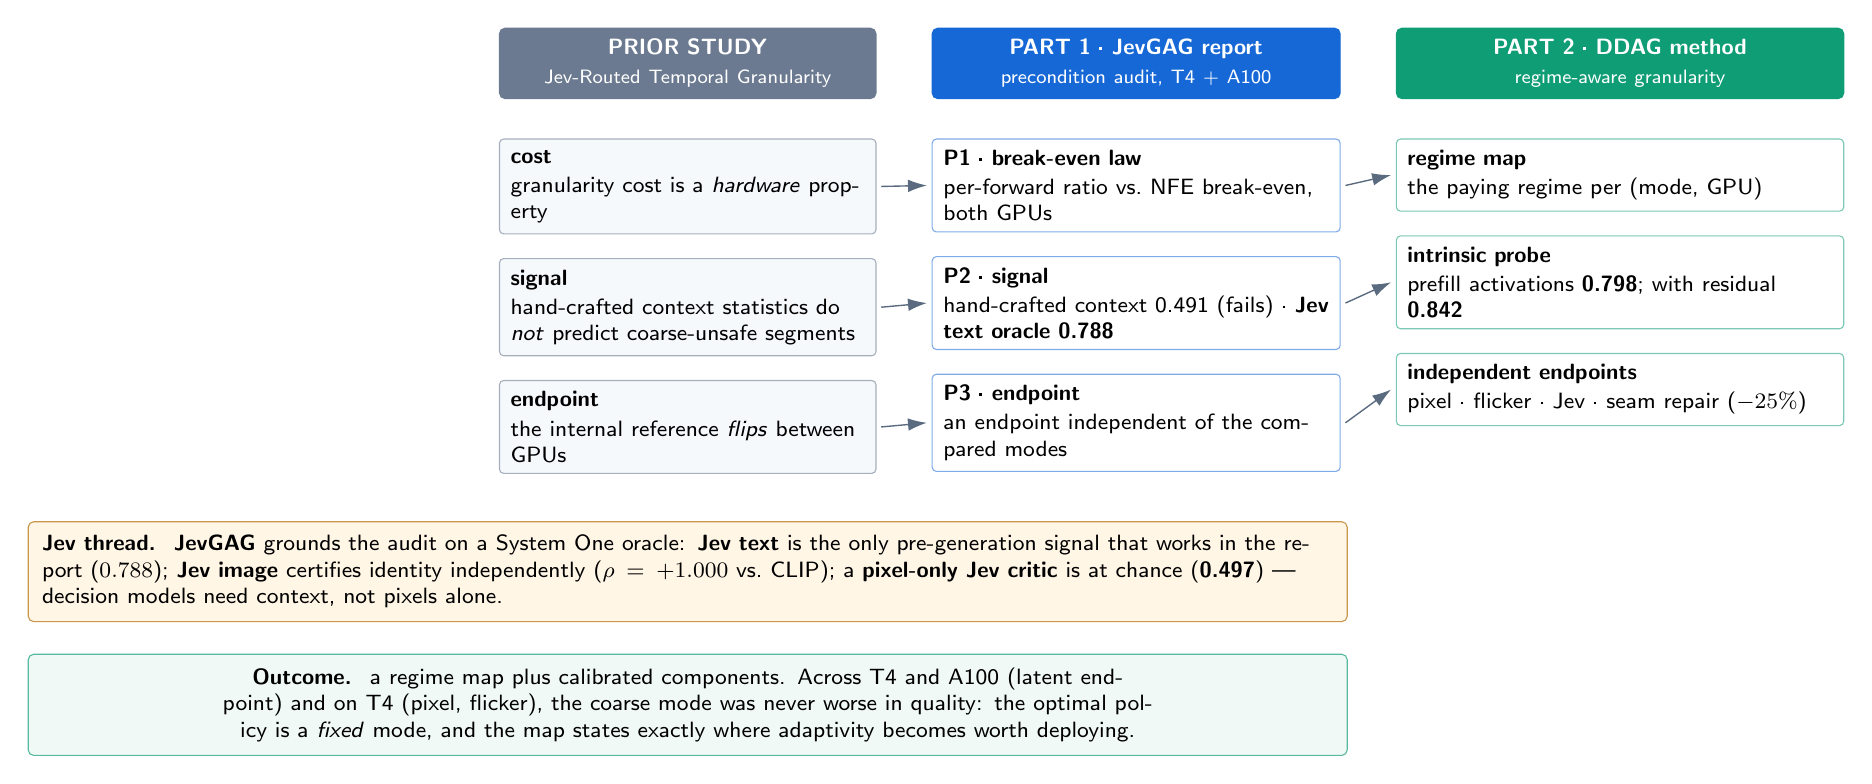
\begin{tikzpicture}[
  font=\footnotesize,
  >={Latex[width=1.6mm,length=2.4mm]},
  hdr/.style={rounded corners=2pt,draw=ink,fill=ink,text=white,align=center,
              inner sep=4pt,minimum height=8mm},
  cell/.style={rounded corners=1.5pt,draw=line,fill=white,align=left,
               inner sep=4pt,minimum height=7mm},
  ar/.style={->,draw=muted,line width=0.5pt},
]

% ---------------- column headers ----------------
\node[hdr,fill=priorc,draw=priorc,text width=4.5cm] (h1)
  {\textbf{PRIOR STUDY}\\[1pt]\scriptsize Jev-Routed Temporal Granularity};
\node[hdr,fill=reportc,draw=reportc,text width=4.9cm,right=7mm of h1] (h2)
  {\textbf{PART 1 \textperiodcentered\ JevGAG report}\\[1pt]\scriptsize precondition audit, T4 + A100};
\node[hdr,fill=methodc,draw=methodc,text width=5.4cm,right=7mm of h2] (h3)
  {\textbf{PART 2 \textperiodcentered\ DDAG method}\\[1pt]\scriptsize regime-aware granularity};

% ---------------- row 1: COST ----------------
\node[cell,text width=4.5cm,draw=priorc!60,fill=rowbg,below=5mm of h1] (l1)
  {\textbf{cost}\\[1pt] granularity cost is a \emph{hardware} property};
\node[cell,text width=4.9cm,draw=reportc!55,below=5mm of h2] (r1)
  {\textbf{P1 \textperiodcentered\ break-even law}\\[1pt] per-forward ratio vs.\ NFE break-even, both GPUs};
\node[cell,text width=5.4cm,draw=methodc!55,below=5mm of h3] (m1)
  {\textbf{regime map}\\[1pt] the paying regime per (mode, GPU)};

% ---------------- row 2: SIGNAL ----------------
\node[cell,text width=4.5cm,draw=priorc!60,fill=rowbg,below=3mm of l1] (l2)
  {\textbf{signal}\\[1pt] hand-crafted context statistics do \emph{not} predict coarse-unsafe segments};
\node[cell,text width=4.9cm,draw=reportc!55,below=3mm of r1] (r2)
  {\textbf{P2 \textperiodcentered\ signal}\\[1pt] hand-crafted context 0.491 (fails) \textperiodcentered\ \textbf{Jev text oracle 0.788}};
\node[cell,text width=5.4cm,draw=methodc!55,below=3mm of m1] (m2)
  {\textbf{intrinsic probe}\\[1pt] prefill activations \textbf{0.798}; with residual \textbf{0.842}};

% ---------------- row 3: ENDPOINT ----------------
\node[cell,text width=4.5cm,draw=priorc!60,fill=rowbg,below=3mm of l2] (l3)
  {\textbf{endpoint}\\[1pt] the internal reference \emph{flips} between GPUs};
\node[cell,text width=4.9cm,draw=reportc!55,below=3mm of r2] (r3)
  {\textbf{P3 \textperiodcentered\ endpoint}\\[1pt] an endpoint independent of the compared modes};
\node[cell,text width=5.4cm,draw=methodc!55,below=3mm of m2] (m3)
  {\textbf{independent endpoints}\\[1pt] pixel \textperiodcentered\ flicker \textperiodcentered\ Jev \textperiodcentered\ seam repair ($-25\%$)};

% row-to-row arrows removed on purpose: cost / signal / endpoint are PARALLEL
% preconditions, not a sequence; only the horizontal limit -> audit -> resolution
% arrows carry meaning.
% column-to-column arrows
\foreach \a/\b in {l1/r1,l2/r2,l3/r3,r1/m1,r2/m2,r3/m3}{
  \draw[ar] ($(\a.east)+(0.6mm,0)$) -- ($(\b.west)-(0.6mm,0)$);
}

% ---------------- JEV THREAD BAND ----------------
\node[rounded corners=2pt,draw=jevc!70,fill=bandbg,align=left,inner sep=5pt,
      text width=16.4cm,below=6mm of l3] (jevband)
  {\textbf{Jev thread.}\;
   \textbf{JevGAG} grounds the audit on a System One oracle:
   \textbf{Jev text} is the only pre-generation signal that works in the report ($0.788$);
   \textbf{Jev image} certifies identity independently ($\rho=+1.000$ vs.\ CLIP);
   a \textbf{pixel-only Jev critic} is at chance (\textbf{0.497}) --- decision models need context, not pixels alone.};

% ---------------- OUTCOME ----------------
\node[rounded corners=2pt,draw=methodc!70,fill=methodc!6,align=center,inner sep=5pt,
      text width=16.4cm,below=4mm of jevband] (out)
  {\textbf{Outcome.}\; a regime map plus calibrated components.
   Across T4 and A100 (latent endpoint) and on T4 (pixel, flicker), the coarse mode was never worse in quality:
   the optimal policy is a \emph{fixed} mode, and the map states exactly where adaptivity becomes worth deploying.};

\end{tikzpicture}
\end{document}
